\documentclass[12pt]{amsart}
\usepackage[margin=1in]{geometry}
\usepackage{hyperref}
\usepackage{natbib}
\usepackage{times}
\usepackage{amsfonts}
\usepackage{amsmath}
\usepackage[psamsfonts]{amssymb}
\usepackage{amstext}
\usepackage{amsthm}
\usepackage{latexsym}
\usepackage{color}
\usepackage{graphicx}
\usepackage{subfig}
\usepackage{enumerate}
\usepackage{enumitem}
\usepackage{url}
\usepackage{comment}
\usepackage{multirow}
\usepackage{hhline}

\makeatletter
\newtheorem*{rep@theorem}{\rep@title}
\newcommand{\newreptheorem}[2]{%
\newenvironment{rep#1}[1]{%
 \def\rep@title{#2 \ref{##1}}%
 \begin{rep@theorem}}%
 {\end{rep@theorem}}}
\makeatother

\hypersetup{
  colorlinks   = true,
  urlcolor     = blue,
  linkcolor    = blue,
  citecolor   = blue
}

\let\Pr\undefined
\def\Rset{\mathbb{R}}
\def\Nset{\mathbb{N}}
\def\vcdim{\text{VCdim}}
\def\pdim{\text{Pdim}}
\DeclareMathOperator*{\E}{\mathbb{E}}
\DeclareMathOperator*{\Pr}{\mathbb{P}}
\DeclareMathOperator*{\argmax}{\rm argmax}
\DeclareMathOperator*{\argmin}{\rm argmin}
\DeclareMathOperator{\sgn}{sgn}
\DeclareMathOperator{\sign}{sign}
\DeclareMathOperator{\supp}{supp}
\DeclareMathOperator{\range}{range}
\DeclareMathOperator{\rank}{rank}
\DeclareMathOperator{\diag}{diag}
\DeclareMathOperator{\Tr}{Tr}
\providecommand{\norm}[1]{\| #1 \|}
\providecommand{\frobp}[2]{\langle#1, #2\rangle_F}
\def\dqed{\relax\tag*{\qed}}

\newcommand{\set}[1]{\{#1\}}
\newcommand{\iprod}[2]{\left\langle #1, #2 \right\rangle}
\newcommand{\h}{\widehat}
\newcommand{\tl}{\widetilde}
\newcommand{\Alpha}{{\boldsymbol \alpha}}
\newcommand{\mat}[1]{{\mathbf #1}}
\newcommand{\be}{\mat{e}}
\newcommand{\bu}{\mat{u}}
\newcommand{\bh}{\mat{h}}
\newcommand{\n}{\mat{n}}
\newcommand{\K}{\mat{K}}
\newcommand{\N}{\mat{N}}
\newcommand{\0}{\mat{0}}
\newcommand{\w}{\mat{w}}
\newcommand{\x}{\mat{x}}
\newcommand{\cB}{\mathcal{B}}
\newcommand{\cL}{\mathcal{L}}
\newcommand{\cX}{\mathcal{X}}
\newcommand{\Ind}{\mathds{1}}
\newcommand{\1}{\mathds{1}}
\newcommand{\R}{\mathfrak{R}}
\newcommand{\e}{\epsilon}
\newcommand{\EQ}{\gets}
\newcommand{\wt}{\widetilde}
\newcommand{\ssigma}{{\boldsymbol \sigma}}
\newcommand{\tts}{\tt \small}
\newcommand{\TO}{\mbox{ {\bf to }}}

\newtheorem{theorem}{Theorem}
\newreptheorem{theorem}{Theorem}
\newtheorem{lemma}[theorem]{Lemma}
\newreptheorem{lemma}{Lemma}
\newtheorem{definition}[theorem]{Definition}
\newtheorem{corollary}[theorem]{Corollary}
\newreptheorem{corollary}{Corollary}
\newtheorem{proposition}[theorem]{Proposition}
\newreptheorem{proposition}{Proposition}

\newenvironment{code}{\begin{tabbing}
    12\=12\=12\=12\=12\=12\=12\=12\= \kill }
  {\end{tabbing}}
\newcommand{\ignore}[1]{}


\title{WikiNet: Wikipedia as a Network}
\author{Chen Zhang (cz1389) \& Guang Yang (gy552)}

\begin{document}

\begin{abstract}
We present the prototype of WikiNet, a relation-based search engine for Wikipedia. A heuristic crawler is built to colloect a small propotion of wikipedia pages. Using the the structural infomation and content of the pages, we model the dataset as a directed weighted graph. Based on this graph, WikiNet carries our similarity based search. So far, two functions are implemented, namely, to search a page's most related pages, and to search the  most related path between a pair of pages. Analysis show that WikiNet provides much higher-quality relations between wikipedia pages than na\"ive BFS strategy. 
\end{abstract}

\maketitle

\section{Introduction}

Wikipedia is so far the largest public online database of knowledge. 
When searching over wikipedia, it is almost certain that there will be a page excatly match the query. 
Aside from the incredibly high precision, wikipedia also enjoys a high degree of diversity. The wikipedia articles are related to other pages through the numerous hyperlinks. 
When reading wikipedia articles, people always follow the links to some other related topics(usually in a depth-first pattern). 
At the end of the day, we can be very far from what we intended in the first place. 

The quality of the relation between connected pages varies drasticly. If a link with poor relation is followed, people may be diverted into a very different field. 

That is where WikiNet starts. We seek to search for high quality relations in wikipedia. 
In Section~\ref{sec:wiki}, we introduce a heuristic crawler that help us collect reasonable amount of kind-of-related wikipedia pages. 
In Section~\ref{sec:net}, we modeled our dataset as directed weighted graph based on the structural information and the content of the pages. 
In Section~\ref{sec:wikinet}, the function of WikiNet is introduced. 
We conclude in Section~\ref{sec:eva}, where we raised an evaluation measurement and discussive the performance of WikiNet against the na\"ive approach. 

\section{The Wiki part: Heuristic crawler}
\label{sec:wiki}
Because of our limited storage and computation resource, it is not feasible for us to traversd and index the whole wikipedia. As a result, heuristic methods are heavily used.

Wikipedia pages have in- and out-links to other pages. Some links are pointing at a highly related page, while others are not. (i.e. The page of \href{https://en.wikipedia.org/wiki/Apple}{apple} the fruit, has a hyper link to \href{https://en.wikipedia.org/wiki/Adam_and_Eve}{Adam and Eve}. However, the word of "apple" doesn't even appear on the latter. In fact, it is \href{https://en.wikipedia.org/wiki/Apple_(symbolism)}{apple} the symbol that is closely related to Adams and Eves. ) So when crawling wikipedia pages, we conduct for- and backwards evaluation and only index the highly related pages. 

\begin{figure}[htb]
\begin{code}
\textsc{HeuristicCrawler}($seed$, $maxDepth$): \\
\> \textsc{Queue} $U$ \\
\> \textsc{Set} $V$ \\
\> $U.\textsc{Push}(\langle seed, 0 \rangle)$ \\
\> \textbf{While} $U.\textsc{NotEmpty}()$: \\
\>\> $ \langle p, depth \rangle \leftarrow U.Pop()$ \\
\>\> \textbf{If} $p$ is closely related to its parent: \\
\>\>\> $V.\textsc{Insert}(p)$ \\
\>\> \textbf{If} $depth < maxDepth$: \\
\>\>\> \textbf{For all} $hyperlink$ in the content of $p$: \\
\>\>\>\> \textbf{If} $hyperlink$ is important in $p$: \\
\>\>\>\>\> $U.\textsc{Push}(hyperlink)$\\ 
\> \textbf{Return} $V$
\end{code}
\caption{Heuristic crawler alogrithm}
\label{al:crawler}
\end{figure}

The algorithm of the heuristic crawller is shown as Fig.~\ref{al:crawler}. In order to guarantee that only the related pages are indexed, we perform forward and backward check. 

\begin{description}
\item[Forward] In order to judge if a $hyperlink$ is important in page $v$, we devloped a scoring mechanism. Each occurrence of the anchor text in the introduction part counts for $3$ point, while others count for $1$ point. $Hyperlinks$ that score \textbf{more than $1$ point} is considered realted. The related pages are added into the Queue
\item[Backward] The forward check guarantees that the page being visited is some how related to its parent. We perform a backward check to guarantee the mutual relation. Again, a scoring mechanism is introduced. Each link back to its parent page counts for $3$ points, and each reference to the title of its parent counts for $1$ point. Only the pages (except the seed) that scores \textbf{at least $3$ points} are indexed. If a page is found irrelevant, it is droped immediately along with the hyperlinks in it. 
\end{description}

This stragety is not perfect. For example, it is common sense that \href{https://en.wikipedia.org/wiki/Deep\_learning}{deep learning} has a lot to do with \href{https://en.wikipedia.org/wiki/Yann\_LeCun}{Yann LeCun}. However, the former wasn't mentioned in the content (literally, not a word) of the latter. In this case, when visiting \href{https://en.wikipedia.org/wiki/Yann\_LeCun}{Yann LeCun} and perform backward check, the page will be marked as irrelevant. Actually, the wikipedia page of  \href{https://en.wikipedia.org/wiki/Yann\_LeCun}{Yann LeCun} is of such a low quality that it is almost isolated. 

We limit the depth of the BFS crawling to $4$ and crawled pages from $4$ different seeds. A brief discription of the 

\begin{table}[htb]
\centering
\begin{tabular}{|l|r|r|}\hline
seed & \# visted pages & \# indexed pages \\ \hline
\href{https://en.wikipedia.org/wiki/Apple}{\textsf{https://en.wikipedia.org/wiki/Apple}} & 13956 & 6619 \\ \hline
\href{https://en.wikipedia.org/wiki/Apple\_Inc.}{\textsf{https://en.wikipedia.org/wiki/Apple\_Inc.}} & 14929 & 6050 \\ \hline
\href{https://en.wikipedia.org/wiki/Artificial\_intelligence}{\textsf{https://en.wikipedia.org/wiki/Artificial\_intelligence}} & 27123 & 12682 \\ \hline
\href{https://en.wikipedia.org/wiki/New\_York\_University}{\textsf{https://en.wikipedia.org/wiki/New\_York\_University}} & 17688 & 6769 \\ \hline 
\end{tabular}
\caption{A discription of the dataset we collected. }
\label{tbl:dataset}
\end{table}

We only conduct experiment on the two apples. You may search using the keyword "apple" to find out which one is currently running. 


\section{The Net part: Directed weighted graph}
\label{sec:net}
Now that Wikipedia is an online database, the system is by nature a complex network, where artibles are the nodes, and hyperlinks the edges. We build a graph from the dataset. We used TF-IDF to index the main content of the pages and marked the weight of the edges using the cosine coefficent between the two pages. We end up with a directed weighted graph. We visualized the graph resulted from 3 of the 4 datasets. 

\begin{figure}[htb]
\centering
\subfloat[\href{https://en.wikipedia.org/wiki/Apple}{apple}]{
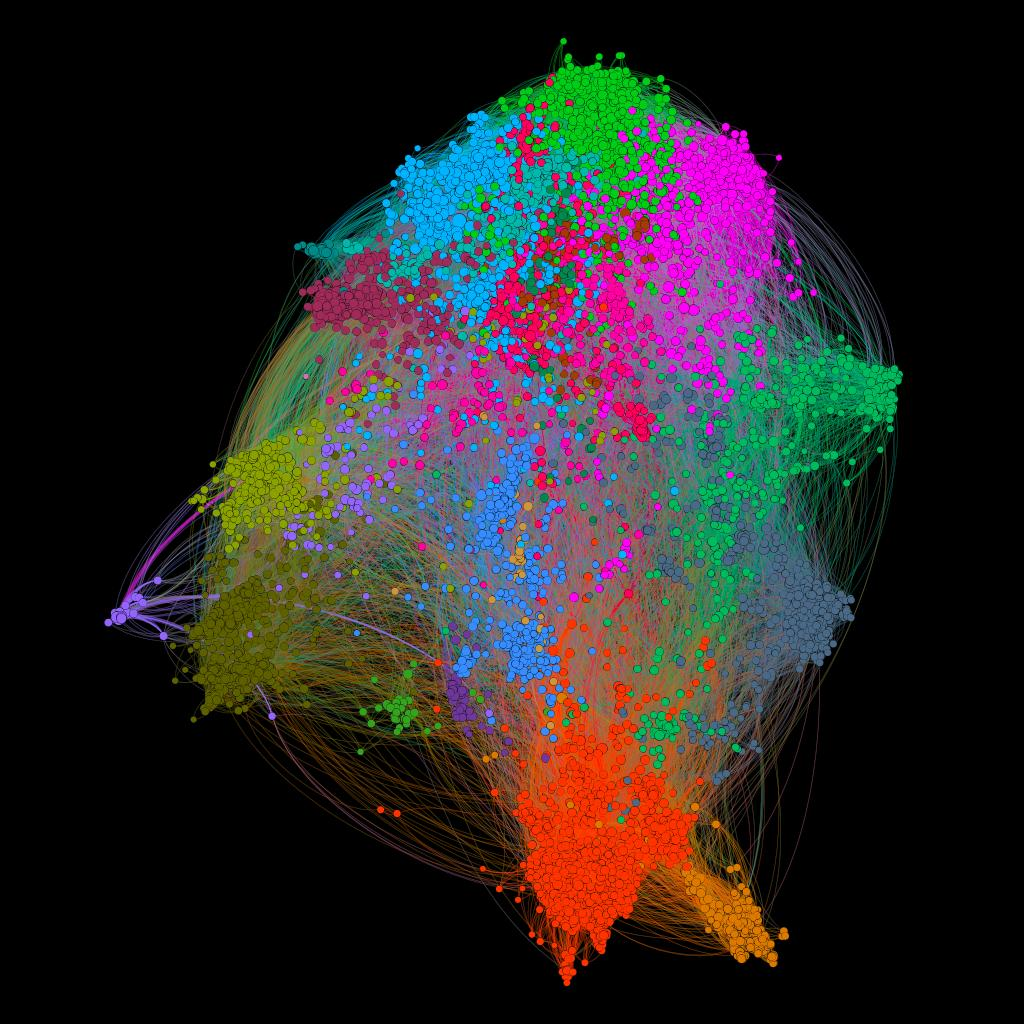
\includegraphics[height=2in]{apple}
\label{fig:net.apple}
}
~
\subfloat[\href{https://en.wikipedia.org/wiki/Apple_Inc.}{Apple Inc.}]{
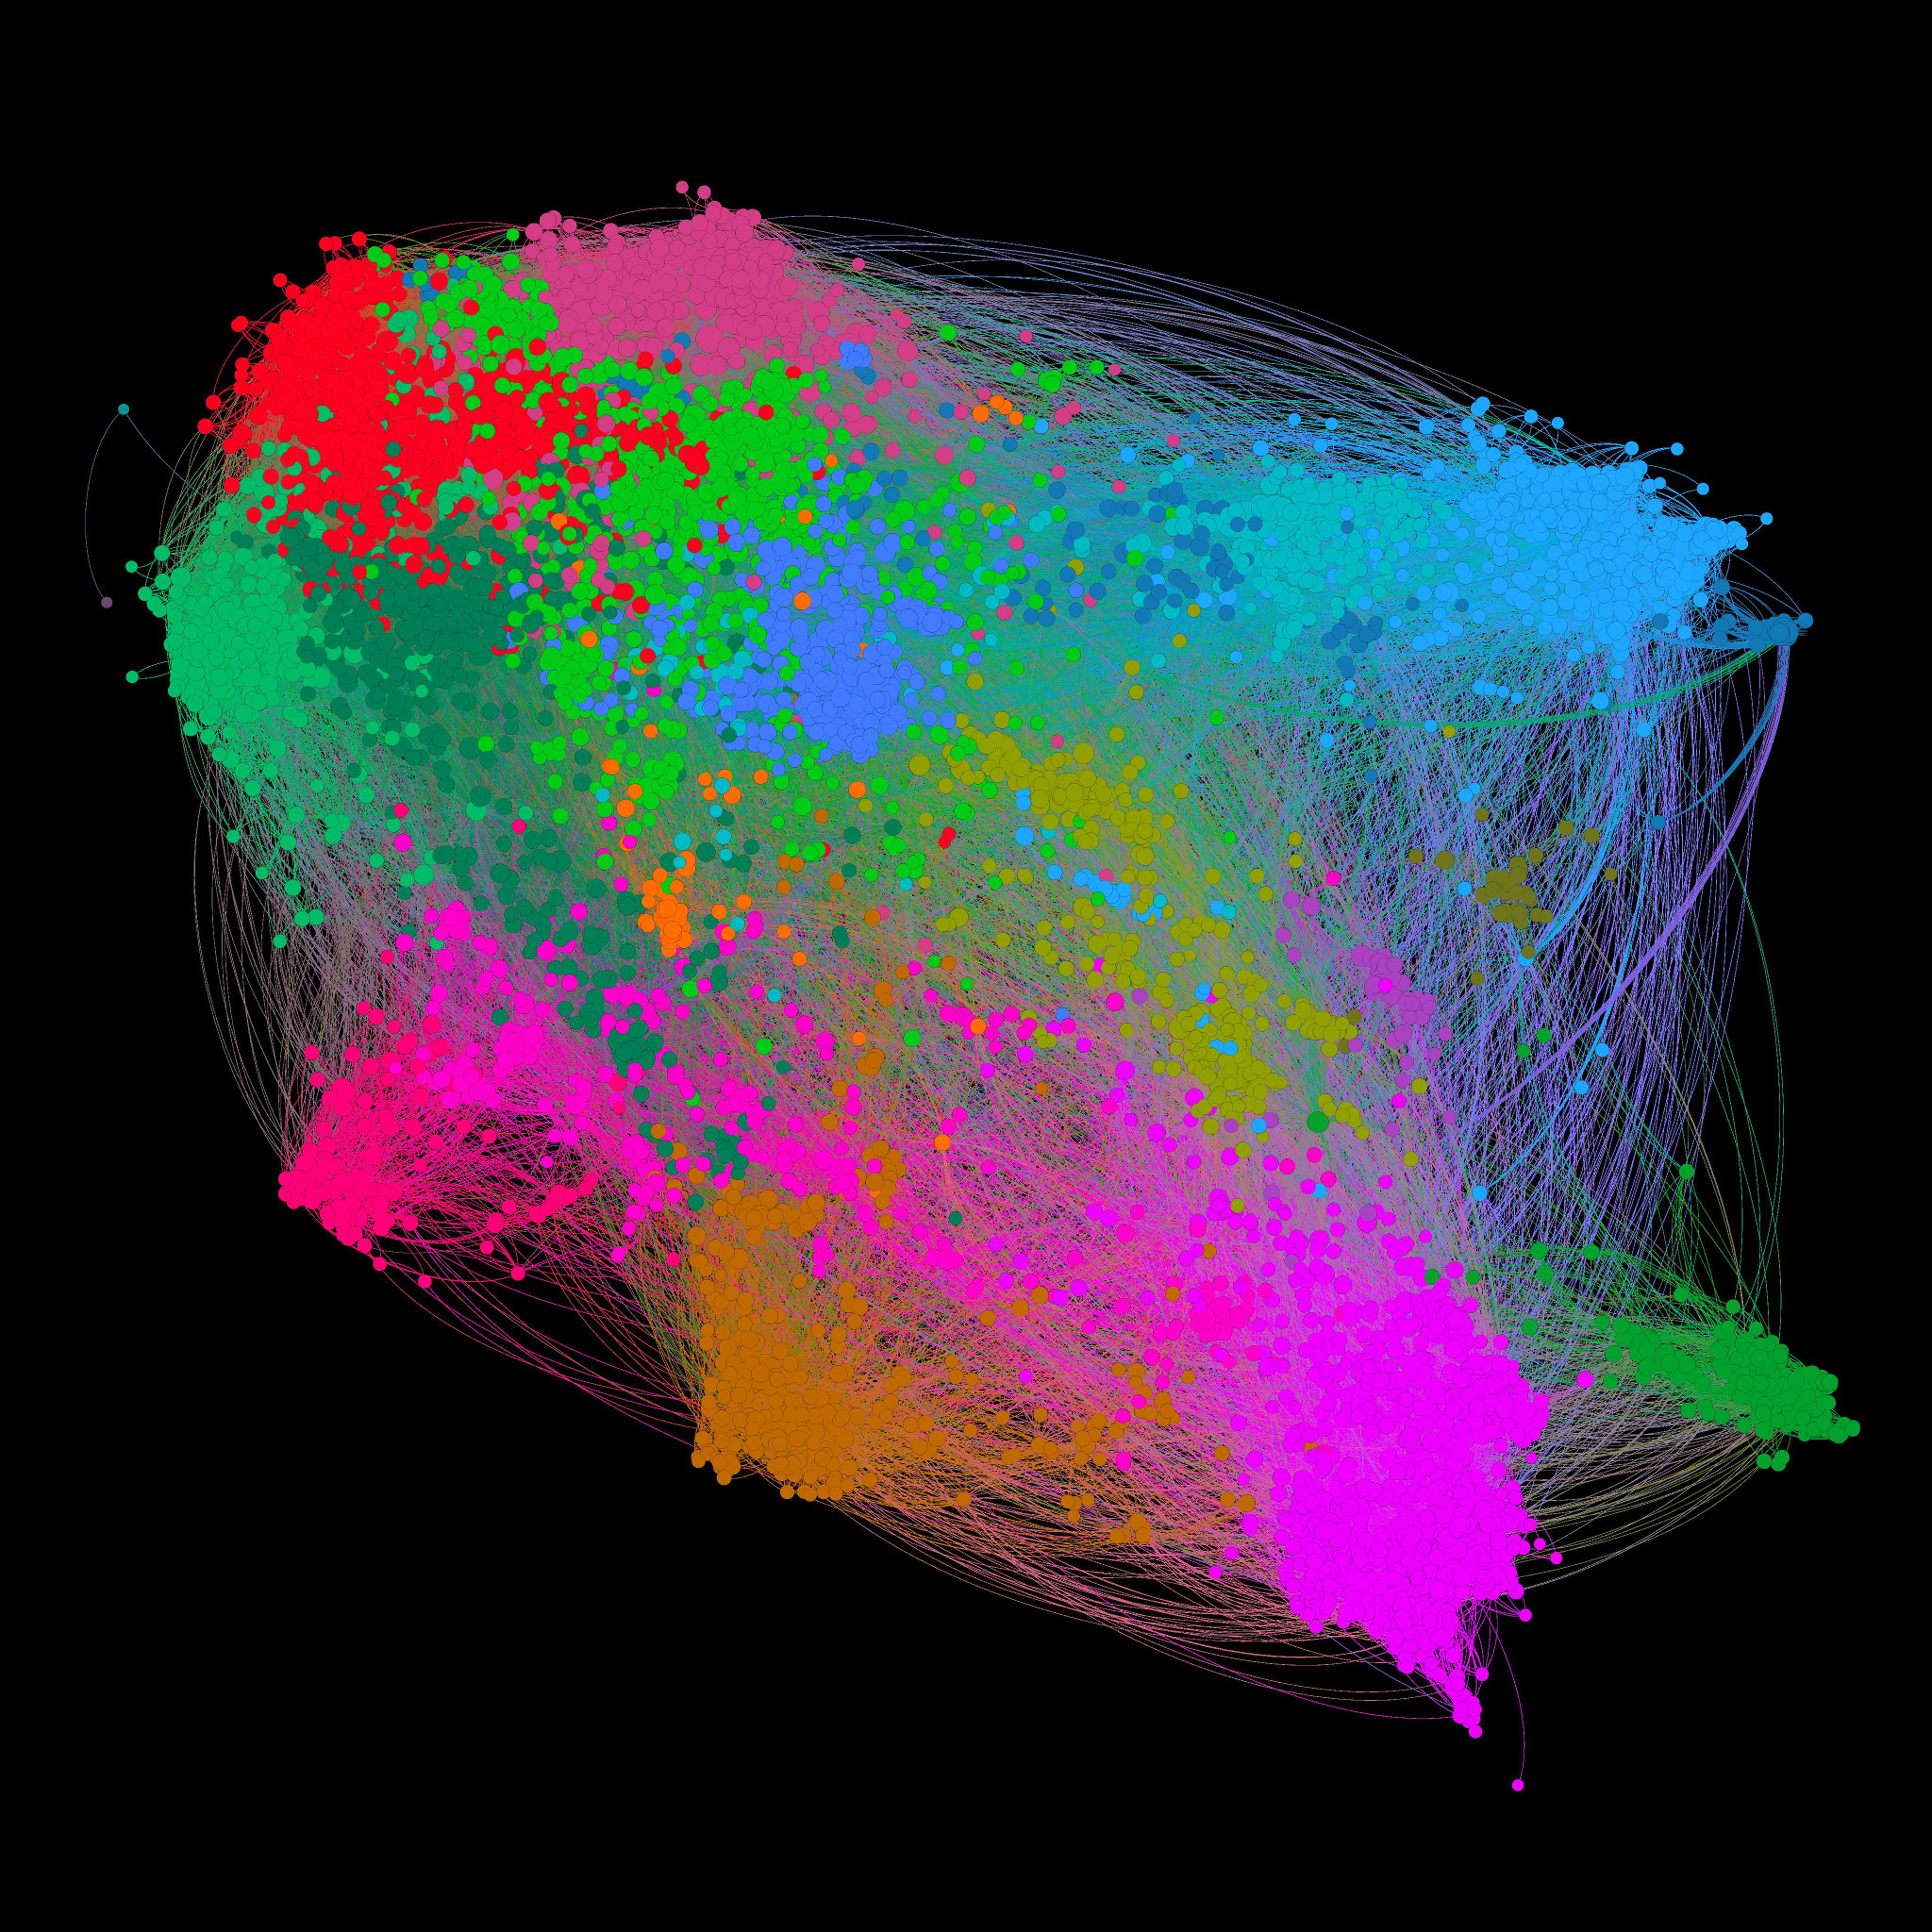
\includegraphics[height=2in]{inc}
\label{fig:net.inc}
}
~
\subfloat[\href{https://en.wikipedia.org/wiki/Artificial\_intelligence}{Artificial\_intelligence}]{
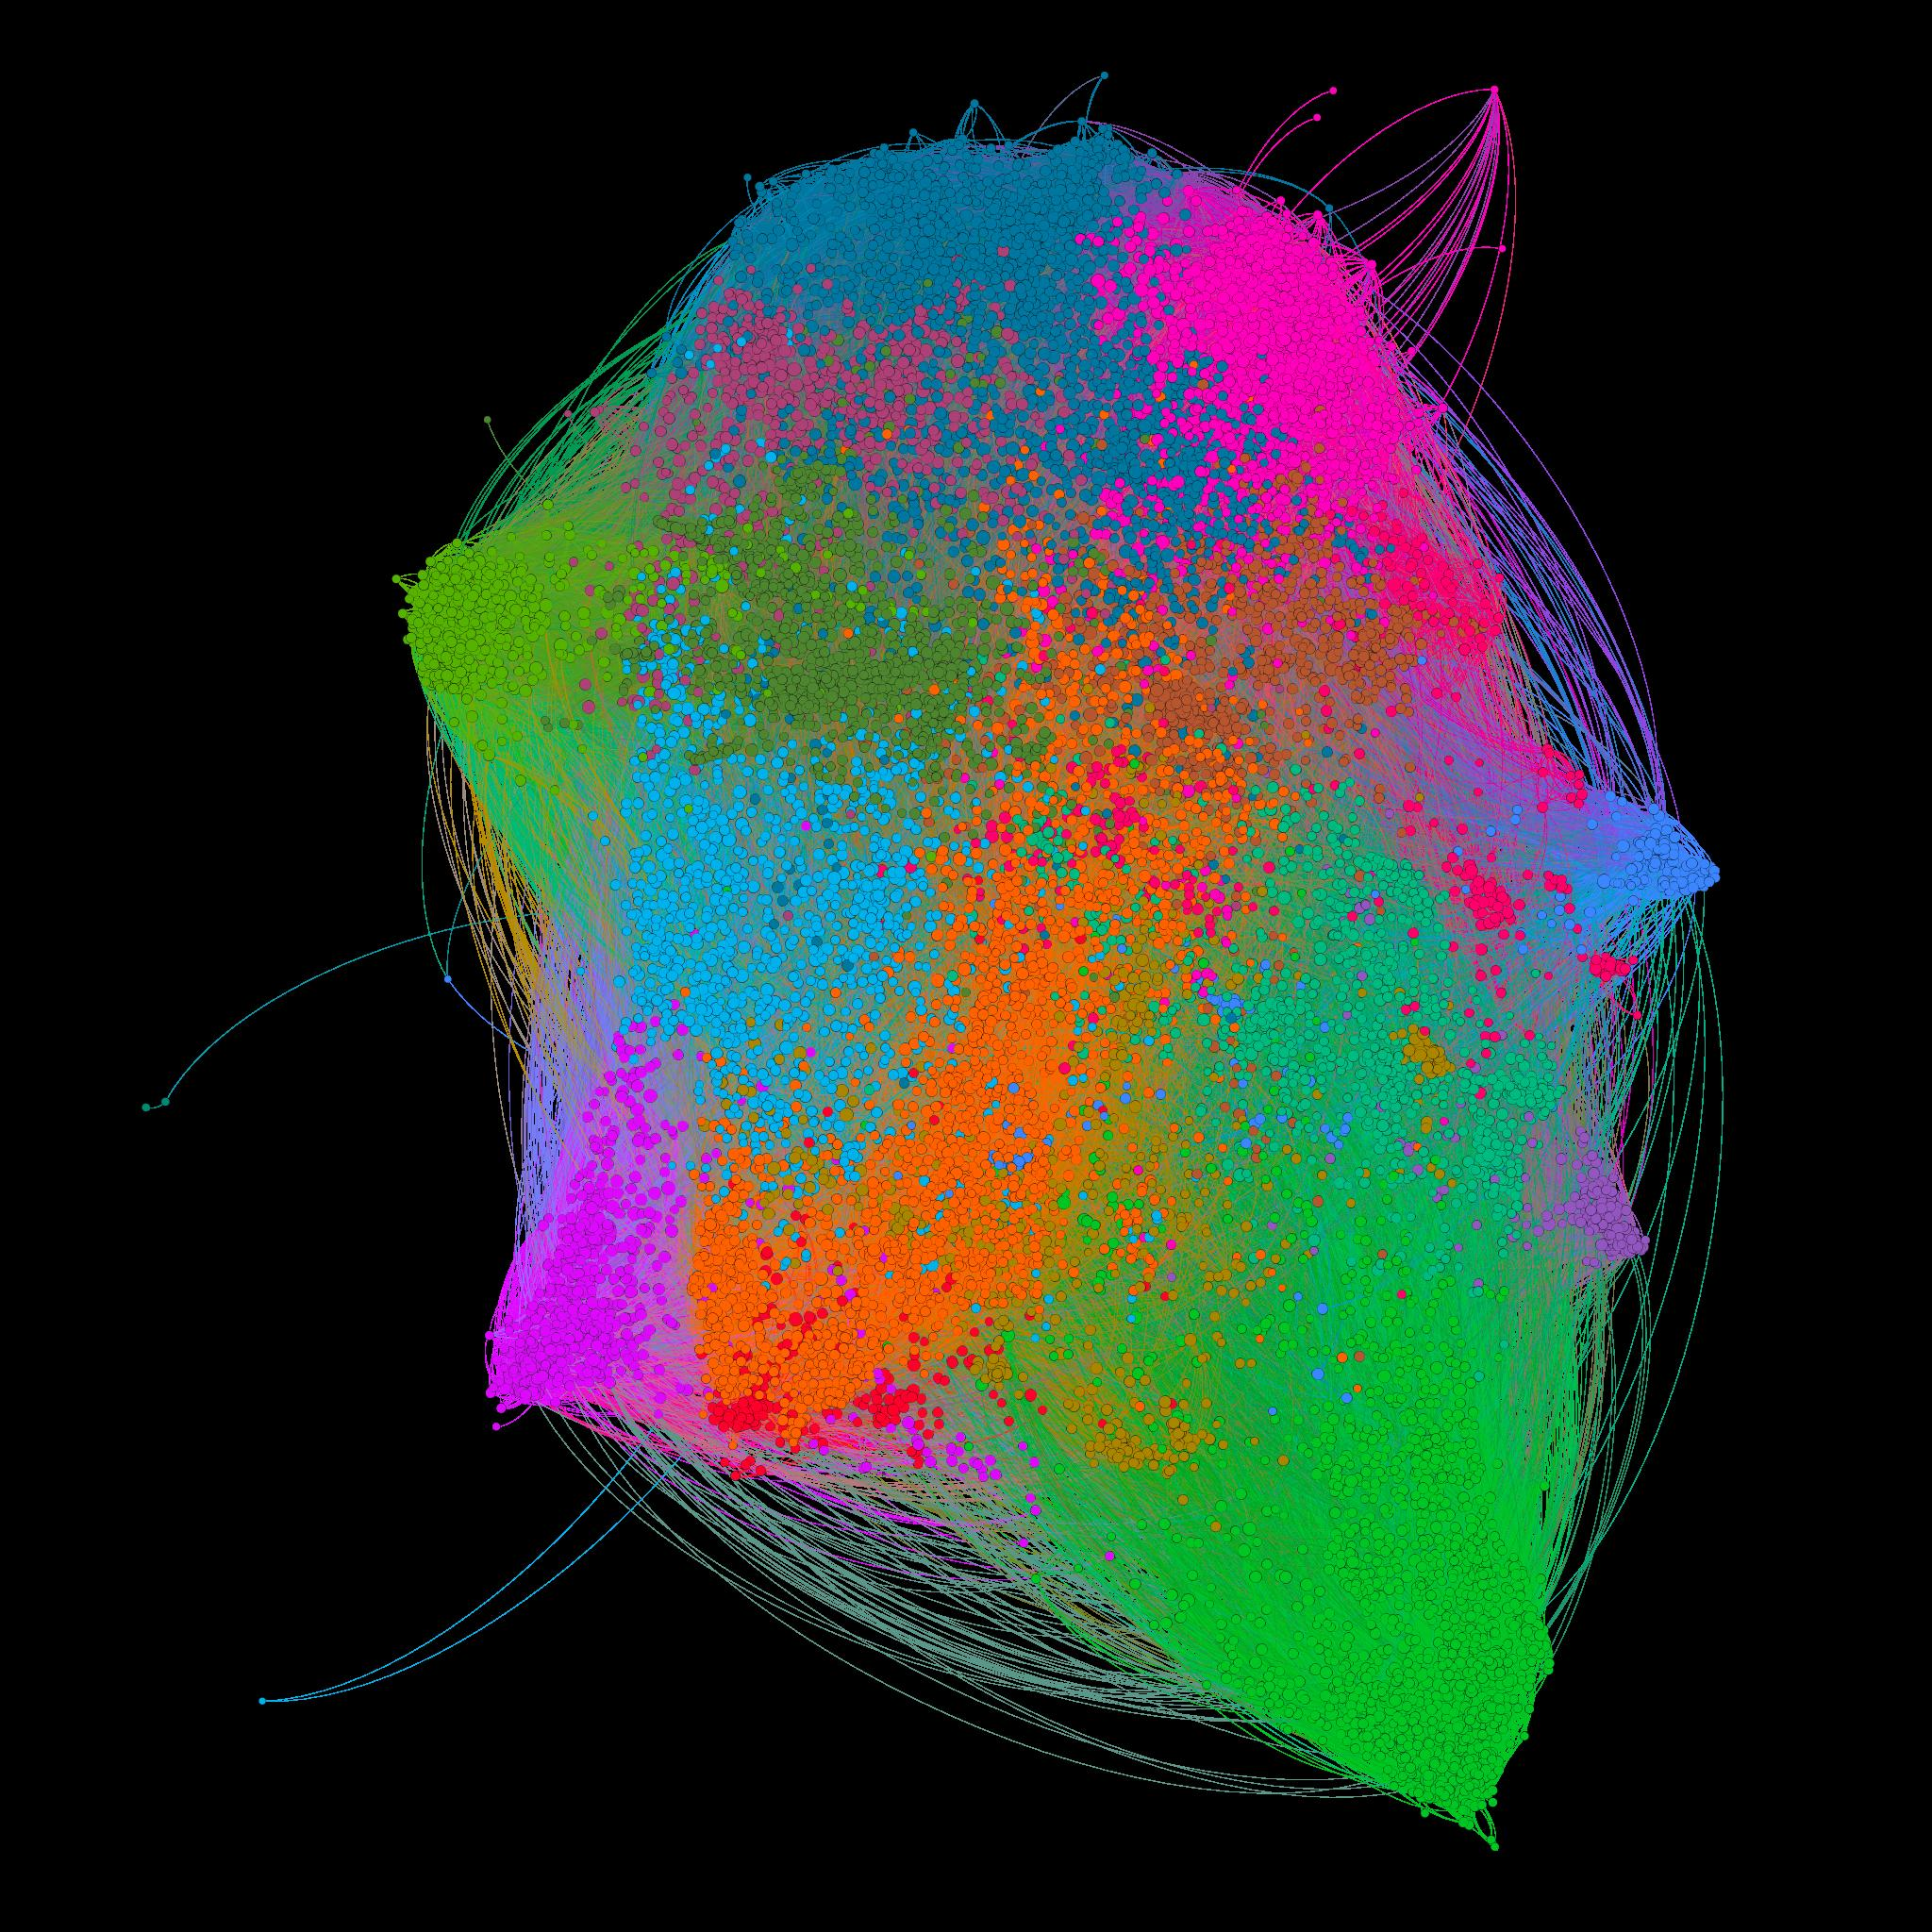
\includegraphics[height=2in]{ai}
\label{fig:net.ai}
}
\caption{This is an illustration of the graph corresponding to the 3 of the dataset. Nodes of the same color fall into the same cluster based on a modularity-based community detection algorithm (the Louvain method).}
\label{fig:net}
\end{figure}

Finding the most related page or path is similar to the Longest Simple Path problem, which is NP-hard. Luckily, in our case, the weight of the edges are between 0 and 1. If we define the weight of a path as the  multiplication of the cosine coefficent of consecutive pair of pages on the path, 
\[
W(\mathcal{S}) = \prod_{i = 0}^{length(\mathcal{S})}w_{i, i+1}, \hbox{ where } \mathcal{S}=\langle v_0, v_1, \dots, v_{length(\mathcal{S})} \rangle, 
\]
which is a reasonable definition, the weight of a path decreases monotonously as we traverse the graph. This definition of the weight excludes loop in the path by definition. In this case, a smart modification to the widely-used all pair shortest path algorithm is sufficient to solve our problem. We therefore define the closeness between a pair of pages as the largest weight of all paths between them.
\[
D(v_i,v_j) = \max_{\mathcal{S} \in \{\langle v_i, \dots, v_j \rangle \}} W(\mathcal{S}) 
\]
The algorithm to solve the problem is given in Fig~\ref{al:dist}. It is based on the Floyd-Warshall algorithm. 
\begin{figure}
\begin{code}
\textsc{MostRelatedPath}$(cosineCoefficient)$: \\
\> $D = cosineCoefficient$ \\
\> $N=D.\textsc{size}$ \\
\> $M = \big[ M_{i,i} =i \big], i\in\{1,\dots,N\}]$ \\
\> \textbf{For} $ k \leftarrow 1,\dots, N$ : \\
\>\> \textbf{For} $ i \leftarrow 1,\dots, N$ : \\
\>\>\> \textbf{For} $ j \leftarrow 1,\dots, N$ : \\
\>\>\>\> \textbf{If} $D_{i,j} < D_{i,k} \times D_{k,j} $: \\
\>\>\>\>\> $D_{i,j} \leftarrow D_{i,k} \times D_{k,j}$ \\
\>\>\>\>\> $M_{i,j} \leftarrow k $ \\
\> \textbf{Return} $D,M$
\end{code}
\caption{Algorithm for all-pair most related path based on Floyd-Warshall}
\label{al:dist}
\end{figure}


\section{The WikiNet}
\label{sec:wikinet}
WikiNet is a relation-based search engine for wikipedia, where the records are too finely ground to tolerate any ambigurity, where diversity is implemented through the links between related articles. 
WikiNet makes uses of both the structure of wikipedia, and the content of it to carry out searching for relation among wikipedia pages. 

So far, we provide two search functions. 
\begin{enumerate}[label=\arabic*.]
\item Match the keywords with the most related wikipedia page in our dataset, then list the top 20 most related children pages and the top 20 most related parent pages.
\item Take a pair of keywords. Match them with the most related wikipedia page in our dataset respectively. Then return the most related path bewteen the two pages. 
\end{enumerate}
The matching is done by firstly match the keywords with the titiles in the dataset. If no match is found, then the keywords are matched with the content. If nothing is archived, then a default page (very likely the seed) is matched. 

For example, in the apple\_inc dataset, the keyword of ``stanford'' will be matched with \href{https://en.wikipedia.org/wiki/Stanford,\_California}{Stanford, California} (the word of ``california'' may have a smaller score than ``university'', so \href{https://en.wikipedia.org/wiki/Stanford\_University}{Stanford University} ranks lower). However, the keyword of ``yann lecun'' will be matched with \href{https://en.wikipedia.org/wiki/Deep\_learning}{deep learning}, because \href{https://en.wikipedia.org/wiki/Yann\_LeCun}{Yann LeCun} is not indexed in the data base. 

\section{Evaluation}
\label{sec:eva}
It is hard to evaluate a search engine. However, since WikiNet is working on the relation between wikipedia pages, we managed to figure out a reasonable measurement. 

For a source page, each page in the returned list several hops away (in the means of all-pair shortest path in a graph).  

Consider the na\"ive way of doing relation search. The most simple yet somehow reasonable way is to do na\"ive breadth-first search. In this case, in response to a query matched with page $q$, the na\"ive strategy will return a list of pages visited in a BFS fashion starting from the source page. 
In comparison, WikiNet returns the destinations of the 20 most related paths starting from the source. 

Denote the documents returned by the na\"ive strategy $ \mathcal{N}(q)=\{d_{q,i}\} $. Use $\mathcal{D}(d_{q,i})$  to mark the depth of document $d_i$ in the BFS tree rooted at $q$. Denote the list returned by WikiNet as $\mathcal{R}(q)=\langle r_{q,1},r_{q,2},\dots, r_{q,20}\rangle$

If we take the WikiNet result as a reference, the recall of the na\"ive stratergy can be represented as 
\[
Recall(q,k) = \frac{1}{\sigma(q,k)}
\huge|
\big[\bigcup_{i = 1}^{\sigma(q,k)} r_{q,i} \big]
\bigcap
\{ d_{q,j} \in \mathcal{N}(q) | \mathcal{D}(d_{q,j}) <= k \} 
\huge|,
\]
where $\sigma(q,k) = \min\{20,\big| \{ d_{q,j} \in \mathcal{N}(q) | \mathcal{D}(d_{q,j}) <= k \} \big|\}$, which means the number of pages within $k$ hops from $q$. The recall equation measures how many of the top $\sigma(q,k)$ pages are at most $k$ hops from $q$. 

We measured every of the $6050$ pages in the apple\_inc dataset. Since the dataset has only 4 layers, and we only return the top 20 pages, we consider $k\in \{1,2,3\}$ to be reasonalbe. 
We plot the CDF of $Recall(q,k): \forall q, \forall k \in \{1,2,3\}$ as Fig~\ref{fig:cdf}. 
\begin{figure}[htb]
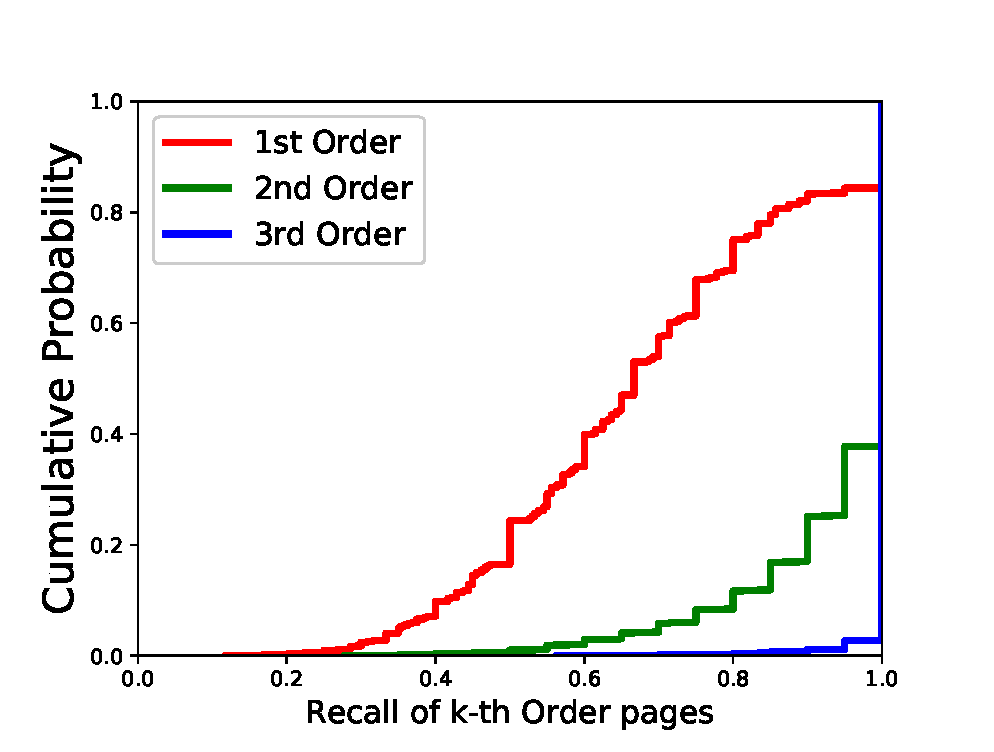
\includegraphics[height=3in]{ratio}
\caption{CFD for $Recall(q,k)$}
\label{fig:cdf}
\end{figure}

As we can see, only in less than $20\%$ of the cases are the top $\sigma(q,1)$ results from WikiNet is fully overlap with the first order pages. In more than $40\%$ of the cases, the top $\sigma(q,1)$ results from WikiNet only contains $60\%$ of the first order pages. Even when it comes to second order pages, there are still around $40\%$ of the cases where some of the top $\sigma(q,2)$ (usually 20) results are at least $3$ hops away. 

We are confident that WikiNet provide content of high quality and diversity. 
\end{document}

